\documentclass[10pt,a4paper]{article}
\usepackage[utf8]{inputenc}
\usepackage[spanish]{babel}
\usepackage{amsmath}
\usepackage{amsfonts}
\usepackage{amssymb}
\usepackage{graphicx}
\usepackage[left=2cm,right=2cm,top=2cm,bottom=2cm]{geometry}

\begin{document}

\begin{titlepage}
\title{\textbf{{\Huge Práctica 2 SATD}}}
\author{
	Pedro Allué Tamargo (758267)
	\and
	Juan José Tambo Tambo (755742)
	\and
	Jesús Villacampa Sagaste (755739)
}
\date{\today}
\clearpage\maketitle
\thispagestyle{empty}
\tableofcontents
\end{titlepage}

\section{Ejercicio 1}

Para diferenciar entre los diferentes nodos de tipo \textit{Row Filter}, se han creado dos tablas tal y como se indica en el guión. 
\begin{itemize}
\item\textit{Row Filter}: Permite filtrar elementos de la tabla a partir de una cadena o una expresión regular.
\item\textit{Nominal Row Filter}: Se puede filtrar manualmente a partir de los atributos de la tabla o mediante expresiones regulares.
\item\textit{Reference Row Filter}: Permite filtrar el contenido de una tabla a partir de una segunda tabla. Para ello, se selecciona la columna deseada de cada tabla para realizar una operación \emph{``join''} entre ambas. También permite realizar un \emph{``join''} con la condición inversa (\textit{exclude}).  
\end{itemize}

\section{Ejercicio 2}

Para verificar que la columna \textit{Ránking} es de tipo \textit{String}, se selecciona esa columna desde la  pre visualización del fichero y se escoge el tipo de dato correspondiente. Desde ahí también se puede modificar el nombre de la columna. \\
Para poder eliminar los comentarios, se deben de modificar las columnas correspondientes añadiendo '//' al principio de las mismas para que sean de tipo comentario \textit{Java}. Desde la previsualización de \textit{Knime}, se selecciona la casilla \textit{Java-Style comments} para poder ignorar los mismos.\\
La columna \textit{class} se puede eliminar añadiendo un elemento de \textit{Column Filter} con el cual se introduce esta columna en el apartado de \textit{exclude}.\\
Si se desea escribir un nuevo fichero CSV, se debe añadir un nuevo componente \textit{CSV writer}. En configuración del módulo se selecciona el tipo de separador, la ruta donde debe escribir el archivo y que se incluya la cabecera con la opción \textit{write column header}.

\section{Ejercicio 3}

En este ejercicio, la modificación del nombre de la columna "marcas" se ha realizado añadiendo un nodo \textit{column rename} a continuación de \textit{CSV reader} (mediante el cual se lee el archivo "data1Nuevo.csv"). \\
Si se desea filtrar las filas con el campo comments = "average", se debe añadir un nuevo nodo \textit{Nominal Value Row Filter}. Se selecciona la columna \textit{comments} y en la seccion de \textit{include} se busca el valor \textit{average}. La columna \textit{ranking} se elimina con el nodo \textit{column filter}.\\
Para la escritura final, se introduce un nodo \textit{CSV writer} y se configura con el modo \textit{append} (se debe indicar que el archivo ya existe), y tabulador como carácter delimitador.

\newpage
\section{Ejercicio 4}

Basándonos en el ejemplo de árbol de decisiones de \textit{Knime}, se ha creado un \textit{Workflow} de árbol de decisión para clasificar las muestras de vinos. 
Para leer el archivo se utiliza el nodo \textit{File Reader}. Se añade un nodo \textit{Partitioning} con el que se selecciona la cantidad de datos de entrenamiento (el 80\%{}).\\
Seguidamente se añade un nodo \textit{Decision Tree Learner}. Para evitar errores con este nodo, se debe modificar la columna \textit{class} desde el nodo lector de archivos e indicar que es de tipo \textit{String}. Posteriormente se incorpora un nodo \textit{Decision Tree Predictor} el cual ``predice'' los valores.\\
Por último, se añade el nodo \textit{Scorer} para poder observar las predicciones realizadas. Los resultados obtenidos son los siguientes:
\begin{figure}[h!]
	\centering
	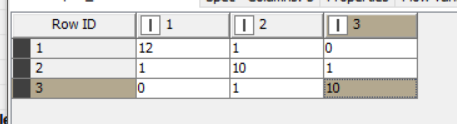
\includegraphics[scale=0.7]{images/prediction.png}
	\caption{Matriz de confusión del árbol de decisión entrenado con el 80\%{} de los datos.}
	\label{fig:prediction} 
\end{figure}

El siguiente cuadro (\ref{tab:ej4_80porcent}) muestra los resultados de ejecutar el \emph{workflow} con un volumen de datos al 80\%{} con 10 iteraciones:

\begin{table}[h!]
\centering
\begin{tabular}{|l|l|l|ll}
\cline{1-3}
\multicolumn{1}{|c|}{\textbf{Clase}} & \multicolumn{1}{c|}{\textbf{Positivos confirmados}} & \multicolumn{1}{c|}{\textbf{Falsos negativos}} & \multicolumn{1}{c}{\textbf{}} &  \\ \cline{1-3}
\textbf{1}                       &         0.91221                       &       0.08778                         &                               &  \\ \cline{1-3}
\textbf{2}                       &         0.93633                       &       0.06366                         &                               &  \\ \cline{1-3}
\textbf{3}                       &         0.94682                       &       0.05317                         &                               &  \\ \cline{1-3}
\end{tabular}
\caption{Cuadro de datos comparativos para el caso de entrenamiento con el 50\%{} de los datos. Los resultados están en tanto por 1.}
\label{tab:ej4_80porcent}
\end{table}

Si se entrena el árbol de decisión con un volumen de datos inferior al 80\%{} se obtienen los siguientes resultados (cuadros \ref{tab:ej4_50porcent} y \ref{tab:ej4_20porcent}):

\begin{table}[h!]
\centering
\begin{tabular}{|l|l|l|ll}
\cline{1-3}
\multicolumn{1}{|c|}{\textbf{Clase}} & \multicolumn{1}{c|}{\textbf{Positivos confirmados}} & \multicolumn{1}{c|}{\textbf{Falsos negativos}} & \multicolumn{1}{c}{\textbf{}} &  \\ \cline{1-3}
\textbf{1}                       &         0.92442                       &       0.07557                         &                               &  \\ \cline{1-3}
\textbf{2}                       &         0.85028                       &       0.14971                         &                               &  \\ \cline{1-3}
\textbf{3}                       &         0.89869                       &       0.10130                         &                               &  \\ \cline{1-3}
\end{tabular}
\caption{Cuadro de datos comparativos para el caso de entrenamiento con el 50\%{} de los datos. Los resultados están en tanto por 1.}
\label{tab:ej4_50porcent}
\end{table}

\begin{table}[h!]
\centering
\begin{tabular}{|l|l|l|ll}
\cline{1-3}
\multicolumn{1}{|c|}{\textbf{Clase}} & \multicolumn{1}{c|}{\textbf{Positivos confirmados}} & \multicolumn{1}{c|}{\textbf{Falsos negativos}} & \multicolumn{1}{c}{\textbf{}} &  \\ \cline{1-3}
\textbf{1}                       &         0.94393                       &       0.05606                         &                               &  \\ \cline{1-3}
\textbf{2}                       &         0.81067                       &       0.18932                         &                               &  \\ \cline{1-3}
\textbf{3}                       &         0.79701                       &       0.20298                         &                               &  \\ \cline{1-3}
\end{tabular}
\caption{Cuadro de datos comparativos para el caso de entrenamiento con el 20\%{} de los datos. Los resultados están en tanto por 1.}
\label{tab:ej4_20porcent}
\end{table}

Por lo tanto, al compararse estos datos (cuadros \ref{tab:ej4_50porcent} y \ref{tab:ej4_20porcent}) con los obtenidos en una ejecución entrenada con el 80\%{} de los datos se llega a la conclusión de que con el 80\%{} de los datos se obtienen mejores resultados, por encima del 90\%{} en identificación de positivos y con un fallo inferior al 10\%{} en falsos negativos.

\newpage
\section{Ejercicio 5}
Como se pide en el enunciado, a partir del ejercicio 4, se modifica para esta vez entrenar la muestra con un perceptrón multicapa. Por tanto, se cambia el nodo \emph{Decision Tree Learner} por \emph{RProp MLP Learner}, así como el nodo \emph{Decision Tree Predictor} por \emph{MultiLayerPerceptron Predictor}. Además, se añade un nodo \emph{Normalizer} antes de hacer el particionado de los datos. 
Los resultados han sido los siguientes:

\begin{table}[h!]
\centering
\begin{tabular}{|l|l|l|ll}
\cline{1-3}
\multicolumn{1}{|c|}{\textbf{Clase}} & \multicolumn{1}{c|}{\textbf{Positivos confirmados}} & \multicolumn{1}{c|}{\textbf{Falsos negativos}} & \multicolumn{1}{c}{\textbf{}} &  \\ \cline{1-3}
\textbf{1}                       &         1                       &       0                         &                               &  \\ \cline{1-3}
\textbf{2}                       &         0,94432 
&       0,05567 
&                               &  \\ \cline{1-3}
\textbf{3}                       &         0,96087                       &       0,03912                         &                               &  \\ \cline{1-3}
\end{tabular}
\caption{Cuadro de datos comparativos para el caso de entrenamiento con el 80\%{} de los datos (10 ejecuciones) con un perceptrón multicapa. Los resultados están en tanto por 1.}
\label{tab:ej5_80porcent}
\end{table}

\begin{table}[h!]
\centering
\begin{tabular}{|l|l|l|ll}
\cline{1-3}
\multicolumn{1}{|c|}{\textbf{Clase}} & \multicolumn{1}{c|}{\textbf{Positivos confirmados}} & \multicolumn{1}{c|}{\textbf{Falsos negativos}} & \multicolumn{1}{c}{\textbf{}} &  \\ \cline{1-3}
\textbf{1}                       &         0,98833                       &       0,01166                         &                               &  \\ \cline{1-3}
\textbf{2}                       &         0,92275 
&       0,07724 
&                               &  \\ \cline{1-3}
\textbf{3}                       &         0,99019                       &       0,00980                         &                               &  \\ \cline{1-3}
\end{tabular}
\caption{Cuadro de datos comparativos para el caso de entrenamiento con el 50\%{} de los datos (10 ejecuciones) con un perceptrón multicapa. Los resultados están en tanto por 1.}
\label{tab:ej5_50porcent}
\end{table}

\begin{table}[h!]
\centering
\begin{tabular}{|l|l|l|ll}
\cline{1-3}
\multicolumn{1}{|c|}{\textbf{Clase}} & \multicolumn{1}{c|}{\textbf{Positivos confirmados}} & \multicolumn{1}{c|}{\textbf{Falsos negativos}} & \multicolumn{1}{c}{\textbf{}} &  \\ \cline{1-3}
\textbf{1}                       &         0,95236                       &       0,04763                         &                               &  \\ \cline{1-3}
\textbf{2}                       &         0,88767 
&       0,11232 
&                               &  \\ \cline{1-3}
\textbf{3}                       &         0,95010                       &       0,04989 &                               &  \\ \cline{1-3}
\end{tabular}
\caption{Cuadro de datos comparativos para el caso de entrenamiento con el 20\%{} de los datos (10 ejecuciones) con un perceptrón multicapa. Los resultados están en tanto por 1.}
\label{tab:ej5_20porcent}
\end{table}

Por lo tanto, al compararse estos datos se llega a la conclusión de que con el 80\%{} de los datos se obtienen mejores resultados, por encima del 94\%{} en identificación de positivos y con un fallo inferior al 6\%{} en falsos negativos.

Con el fin de obtener un rendimiento superior, se parte de la base del entrenamiento con el 80\%{} de los datos, ya que ha sido el que mejor rendimiento ha dado y se modifican diversos parámetros. Los parámetros que se pueden modificar son el número de iteraciones, el número de capas ocultas y el número de neuronas por capa. En el entrenamiento inicial los valores eran los siguientes: \\
\begin{itemize}
	\item Número de iteraciones: 100
	\item Capas ocultas: 1  
	\item Neuronas por capa: 10
	
\end{itemize}

Se han realizado diversas pruebas para ajustar estos parámetros y obtener el mejor resultado.\\
\par
\begin{itemize}
	\item Número de iteraciones: 1000
	\item Capas ocultas: 3  
	\item Neuronas por capa: 10
\end{itemize}

\begin{table}[h!]
	\centering
	\begin{tabular}{|l|l|l|ll}
		\cline{1-3}
		\multicolumn{1}{|c|}{\textbf{Clase}} & \multicolumn{1}{c|}{\textbf{Positivos confirmados}} & \multicolumn{1}{c|}{\textbf{Falsos negativos}} & \multicolumn{1}{c}{\textbf{}} &  \\ \cline{1-3}
		\textbf{1}                       &         0,9772                       &       0,0227                         &                               &  \\ \cline{1-3}
		\textbf{2}                       &         0,9565
		&       0,0435 
		&                               &  \\ \cline{1-3}
		\textbf{3}                       &         1                       &      0 &                               &  \\ \cline{1-3}
	\end{tabular}
	\caption{Cuadro de datos comparativos para el caso de entrenamiento con el 80\%{} de los datos (1000 ejecuciones) con un perceptrón multicapa con tres capas ocultas. Los resultados están en tanto por 1.}
	\label{tab:ej5_20porcent_3hidden_1000}
\end{table}

Con estos valores los resultados han mejorado considerablemente, como se observa en el siguiente cuadro.\\

\newpage
\begin{itemize}
	\item Número de iteraciones: 5000
	\item Capas ocultas: 5 
	\item Neuronas por capa: 10
\end{itemize}
\begin{table}[h!]
	\centering
	\begin{tabular}{|l|l|l|ll}
		\cline{1-3}
		\multicolumn{1}{|c|}{\textbf{Clase}} & \multicolumn{1}{c|}{\textbf{Positivos confirmados}} & \multicolumn{1}{c|}{\textbf{Falsos negativos}} & \multicolumn{1}{c}{\textbf{}} &  \\ \cline{1-3}
		\textbf{1}                       &        0,963636364
		                      &       0,036363636
		                                             &                               &  \\ \cline{1-3}
		\textbf{2}                       &         0,953947368
		&       0,046052632 
		&                               &  \\ \cline{1-3}
		\textbf{3}                       &         0,96
		                       &      0,04
		                        &                               &  \\ \cline{1-3}
	\end{tabular}
	\caption{Cuadro de datos comparativos para el caso de entrenamiento con el 80\%{} de los datos (5000 ejecuciones) con un perceptrón multicapa con 5 capas ocultas y 10 neuronas por capa. Los resultados están en tanto por 1.}
	\label{tab:ej5_20porcent_5hidden_5000}
\end{table}

Con estos valores los resultados han mejorado con respecto al inicial pero han empeorado con respecto a los anteriores valores.
\\

\begin{itemize}
	\item Número de iteraciones: 1000
	\item Capas ocultas: 3  
	\item Neuronas por capa: 100
	
\end{itemize}
\begin{table}[h!]
	\centering
	\begin{tabular}{|l|l|l|ll}
		\cline{1-3}
		\multicolumn{1}{|c|}{\textbf{Clase}} & \multicolumn{1}{c|}{\textbf{Positivos confirmados}} & \multicolumn{1}{c|}{\textbf{Falsos negativos}} & \multicolumn{1}{c}{\textbf{}} &  \\ \cline{1-3}
		\textbf{1}                       &        1                      &       0                         &                               &  \\ \cline{1-3}
		\textbf{2}                       &         0,975
		&       0,025 
		&                               &  \\ \cline{1-3}
		\textbf{3}                       &         1                       &      0 &                               &  \\ \cline{1-3}
	\end{tabular}
	\caption{Cuadro de datos comparativos para el caso de entrenamiento con el 80\%{} de los datos (1000 ejecuciones) con un perceptrón multicapa con tres capas ocultas y 100 neuronas por capa. Los resultados están en tanto por 1.}
	\label{tab:ej5_20porcent_3hidden_1000_100}
\end{table}

Con estos valores se han obtenido los mejores resultados, obteniendo casi una efectividad del 100\%, excepto para los elementos de la clase 2. Sin embargo, el modelo tarda más tiempo en entrenar.
\\

En comparación con el método \textit{Tree Learner}, se puede considerar que el \textit{Perceptrón Multicapa} obtiene mejores resultados para cualquier porcentaje de datos entrenados, como se puede observar en los cuadros anteriores. El porcentaje de positivos confirmados supera el 90\%{} salvo en una ocasión, a diferencia de los resultados obtenidos con el \textit{Tree Learner}, los cuales rondan el 80 e incluso 70\%{} de aciertos en algunos casos.\\
Para obtener mayor precisión en los resultados, el programa \textit{Knime} recomendaba el uso de un nodo \textit{Nomalizer} junto al nodo \textit{MLP Learner} para normalizar los datos de entrada mediante el método \textit{Z-Scorer Normalization}.

\end{document}